\section{The hard coating process}

Hydropower runner's blades are typically eroded by cavitation and abrasion
phenomena, resulting in hydraulic profile deformation, thus efficiency
reduction. The High Velocity Oxygen Fuel (HVOF) coating is a preventive
solution for erosion, and creates a lamellar structure. 

The runner's blades HVOF is a 2000~hp power process which consists of
spraying coating particles by an 8~kg spray gun, through a flame with mixed
hazardous gases. To achieve the best coating layer, the spray gun should be at
a fixed 210~mm to 240~mm distance and $90^o \pm 30^o$ angle, in respect to the
metallic surface plane of the blade; the gun should move with 40~m/min speed
along the blade; and the precision (or coating step) should be 3~mm for a
regular full blade cover \cite{li2002effect}. The
common solution which meets the requirements for \textit{ex situ} HVOF coating
is a robotic manipulator with a blade-sized workspace in a fixed position.

\section{The problem}\label{problem}

The problem is to design a robotic system for \textit{in situ}
hydropower runner's blades. The system must overcome turbine's environmental
aspects, such as, the confined space and turbine's access, the slippery and
sloping floor, and the unfriendly atmospheric conditions. A large-sized industrial
robotic manipulator is not suitable for the operation, as the robot
transportation, \textit{in situ} locomotion and placement is not possible due
to robot dimensions.

A bulb type turbine has the following points of interest for solution
development: 1) the variable pitch propeller, or Kaplan \textbf{blades}; 2) the
variable pitch guide vanes, or \textbf{wicket gates}; 3) the \textbf{runner
area}; 4) the \textbf{draft tube}; and 5) an access for regular
maintenance, or \textbf{hatch}. The Jirau's turbine is the case study of EMMA,
thus a 3D CAD model was built with SolidWorks\raisebox{1ex}{\textregistered}
for simulation and solution analysis (Fig.~\ref{fig::ambiente3d}).

\begin{figure}[h!]
\centering
	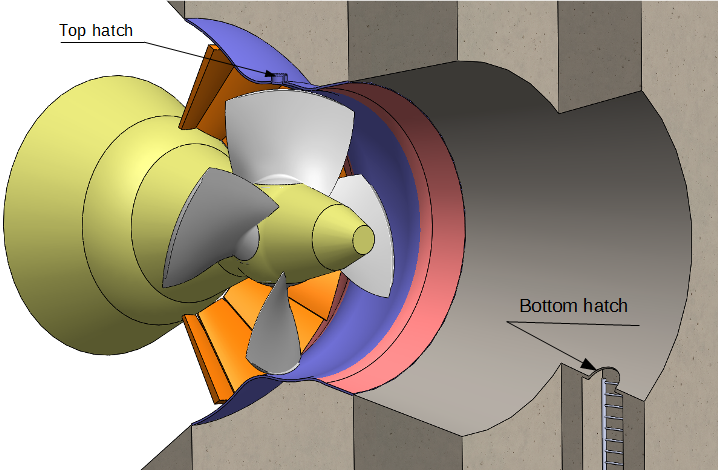
\includegraphics[width=\columnwidth]{figs/problem/ambiente_3d.PNG} 
	\caption{Jirau's hydropower turbine in a 3D CAD model.}
	\label{fig::ambiente3d}
\end{figure}

EMMA must comply with the HVOF requirements, it must overcome the environment
constraints and logistical challenges, such as equipment
and robot transportation, \textit{in situ} locomotion, fixation, and base
rigidity; it must comprise a calibration process for localization and
mapping; and the system must compute the coating strategy, the coating
trajectory planning, and control.

